\documentclass[preprint,12pt]{elsarticle}

\usepackage[T1]{fontenc}
\usepackage[utf8]{inputenc}
\usepackage{lmodern}
\usepackage{microtype}
\usepackage{amsmath}
\usepackage{amssymb}
\usepackage{booktabs}
\usepackage{tabularx}
\usepackage{array}
\usepackage{threeparttable}
\usepackage{graphicx}
\usepackage{tikz}
\usetikzlibrary{arrows.meta,calc,positioning}
\usepackage{float}
\usepackage{caption}
\usepackage[hidelinks]{hyperref}
\usepackage{xurl}

\captionsetup{font=small, labelfont=bf}

\floatstyle{ruled}
\newfloat{algorithm}{t}{loa}
\floatname{algorithm}{Algorithm}

\newcommand{\deltamae}{$\Delta$MAE}
\newcommand{\trimtitlegraphic}[2]{\includegraphics[width=#1,clip,trim=0 0 0 22]{#2}}
\newcommand{\trimdoubletitlegraphic}[2]{\includegraphics[width=#1,clip,trim=0 0 0 34]{#2}}

\journal{Computers \& Geosciences}

\begin{document}

\begin{frontmatter}

\title{An auditable geospatial benchmarking workflow for gridded precipitation products under dense-gauge co-availability}

\author[ua]{Marc Semper}\corref{cor1}
\ead{marc.semper@ua.es}
\author[ua]{Manuel Curado}
\ead{manuel.curado@ua.es}
\author[ua]{Jose F. Vicent}
\ead{jvicent@ua.es}
\author[ps]{Marco Podda}
\ead{marco.podda@unipi.it}

\address[ua]{Department of Computer Science and Artificial Intelligence, University of Alicante, Campus de San Vicente del Raspeig, Ap. Correos 99, E-03080 Alicante, Spain.}

\address[ps]{Department of Computer Science, University of Pisa, Largo Bruno Pontecorvo, 3, 56127 Pisa, Italy.}



\cortext[cor1]{Corresponding author.}

\begin{abstract}
Benchmarking heterogeneous geospatial precipitation sources is difficult because product error, target support, gauge density, spatial alignment, and local alternatives are often conflated. Here we present a reproducible geospatial benchmarking workflow for evaluating gridded precipitation products under dense-gauge co-availability. The workflow defines a common hourly cell--hour universe, harmonizes IMERG, ERA5, and EURADCLIM on the IMERG grid, constructs a within-cell median gauge target from complete AVAMET stations, and compares each gridded source with leave-cell local baselines that exclude gauges from the target cell. It further stratifies performance by rain activity, gauge support, and observable inter-product conflict, allowing gridded-source competitiveness to be assessed conditionally rather than through a single global ranking. Applied to eastern Spain in 2023, the workflow shows that aggregate rankings mask regime-specific behavior: conflict separates low-disagreement screening conditions from rain-active cross-checking conditions, low-conflict gridded gains are dominated by dry-hour composition, stronger local support hardens the benchmark, and source routing has diagnostic value but is sensitive to annual composition. The benchmark is conditional on dense local co-availability and should not be interpreted as standalone gridded-product validation in sparse-gauge regions. The resulting artefact is a reusable computational benchmark rather than a regional product ranking. The workflow and frozen artefacts provide a reusable template for auditable benchmarking of gridded environmental products in dense-observation settings.
\end{abstract}

\begin{keyword}
geospatial benchmarking \sep reproducible workflow \sep gridded precipitation \sep dense gauge networks \sep source disagreement \sep multi-source geospatial evaluation \sep computational geoinformatics
\end{keyword}

\end{frontmatter}


\section{Introduction}

Benchmarking heterogeneous geospatial precipitation sources is a computational problem before it is a product-ranking exercise. This framing follows reproducible geoscience and scientific-computing work that treats data models, executable workflows, provenance, and reusable artefacts as first-class research outputs \citep{pebesma2012rgeoscience,gil2016geosciencepaper,wilson2017goodenough,nuest2021practical}. Gridded products, reanalysis fields, radar-derived estimates, and station observations differ in spatial support, temporal completeness, alignment, error structure, and availability. Without an explicit workflow for defining the evaluation universe and the target support, differences among products can be confounded with differences in gauge density, grid-cell representation, and the local alternatives available at each cell--hour. This issue is especially relevant for precipitation, where gridded products such as IMERG, ERA5, and EURADCLIM are widely used but their apparent value varies across rainfall regime, terrain complexity, and observational support \citep{huffman2020imerg,hersbach2020era5,overeem2023euradclim,tapiador2012gpm,kidd2011status,maggioni2018review,derin2016complexterrain,yu2020highdensity}.

A recurring limitation of validation studies is that they often compress this multidimensional comparison into a single global ranking. Environmental model-evaluation and uncertainty-aware validation studies make a similar point: performance claims depend on the evaluation design, uncertainty treatment, and sampling structure used to construct the comparison \citep{jakeman2006tensteps,refsgaard2007uncertainty,bennett2013performance,roberts2017crossvalidation}. Such rankings are fragile because the measured error of a product depends not only on the product itself, but also on the representativeness of the reference data, the density and placement of gauges, the proxy used for the gridded target, and the regimes over which performance is averaged \citep{tessema2020representativeness,tian2018gaugedensity,tozer2012proxy}. A product that appears competitive in an aggregate benchmark may be less useful in positive-rain hours, high-disagreement situations, or areas where local support is strong. The relevant methodological question is how to construct an auditable benchmark --- one in which every filtering rule, comparator choice, and reported contrast is traceable to a versioned, publicly available input --- that keeps product error, target support, local data availability, and source disagreement separable.

Dense-gauge co-availability makes this question sharper. When many local observations are available, a gridded precipitation product should not only be compared with a station-derived target; it should also be compared with strong local estimators that an operational or analytical workflow could plausibly construct from nearby stations. This requires leakage-controlled local comparators that exclude observations from the target cell while still using surrounding information. It also requires stratification by rain activity, gauge support, and observable disagreement among gridded sources, because the usefulness of broad-coverage products may differ between quiet screening conditions and rain-active local-reference regimes. In this sense, the benchmark brings remote-sensing products and field measurements into a multi-source geospatial evaluation workflow while preserving traceability between inputs, comparators, and reported contrasts \citep{pohl1998datafusion}.

We demonstrate this workflow on the IMERG grid over eastern Spain, using AVAMET as a dense station network and IMERG, ERA5, and EURADCLIM as co-available gridded sources. The target is a within-cell median gauge aggregate in each target IMERG cell and hour, while the local benchmarks are leave-cell inverse-distance baselines built from nearby gauges outside the target cell. The case study is local, but the comparative frame is intended for domains where multiple gridded products are co-available, local observing support is heterogeneous, and users need to decide when broad coverage is sufficient and when dense local evidence should carry more weight \citep{lombardi2024tanaro}. The benchmark is conditional on dense local co-availability and should not be interpreted as standalone gridded-product validation in sparse-gauge regions.

From a computational geoscience perspective, the contribution is not a new precipitation retrieval algorithm, but an auditable benchmarking protocol for aligning heterogeneous gridded and station-based data sources, defining leakage-controlled local comparators, and evaluating source competitiveness under explicit support and disagreement constraints. This study makes four main contributions. First, it provides a reproducible geospatial workflow that harmonizes gridded precipitation sources and station observations on a shared hourly cell--hour universe. Second, it implements a leakage-controlled construction of the local benchmark through leave-cell baselines that exclude all gauges from the target cell. Third, it performs a regime-aware evaluation that separates positive-rain cases, local support gradients, and observable disagreement among products, avoiding reliance on a single aggregate ranking. Fourth, it uses a conflict-gated rule as a diagnostic example of how the benchmark can be converted into an auditable source-routing policy and stress-tested under year-to-year composition shift.

The novelty of this contribution is computational rather than algorithmic: the central result is a reusable benchmark data model and workflow that separates product error, target support, local comparator strength, source disagreement, and reproducibility artefacts into distinct, auditable components. This separation is the methodological contribution; the eastern Spain case study is the demonstration that the workflow functions as intended and produces interpretable, regime-dependent contrasts.

\section{Geospatial data sources and benchmark construction}

\subsection{Study setting and target}

The analysis is conducted on the IMERG grid over eastern Spain, with AVAMET as the dense in situ network. The case study is selected because it combines dense in situ observations with co-available satellite, radar-derived, and reanalysis precipitation products under a common hourly protocol \citep{peino2024westernmed,gomiscebolla2023spain}. This regional setting is meteorologically demanding because western Mediterranean precipitation is shaped by coastal forcing, steep topography, and convective organization \citep{khodayar2021hymex}. Heterogeneous local support, coastal gradients, and terrain contrasts make the domain a useful precipitation-source evaluation stress test. The setting is also societally relevant because Mediterranean intense-rainfall episodes challenge flood vigilance and hydrometeorological monitoring, especially where local network support is uneven \citep{derin2016complexterrain,yu2020highdensity,peino2024westernmed,gomiscebolla2023spain}.

The unit of analysis is the hourly IMERG cell-hour. The target is the median of complete AVAMET stations within the same cell and hour. We use the median because it is generally less sensitive than the mean to isolated station-level spikes and better aligned with cell-scale support than a single station, while acknowledging that robustness is modest when target-cell gauge count is low \citep{tessema2020representativeness,tozer2012proxy}.

\subsection{Gridded products and local benchmarks}

The three gridded products evaluated are IMERG, ERA5, and EURADCLIM \citep{huffman2020imerg,hersbach2020era5,overeem2023euradclim}. They enter the benchmark as harmonized hourly precipitation estimates on the IMERG grid. Their relative behavior is also known to vary across regions and benchmark designs \citep{porcu2014uncertainties,xu2022era5satellite,gomiscebolla2023spain}.

The local comparators are leave-cell inverse distance weighting (IDW) baselines built from AVAMET gauges outside the target cell: 8-neighbor, 64-neighbor, and 64-neighbor within 15 km. We considered three pre-specified leave-cell IDW baselines---nearest-8, nearest-64, and nearest-64 within 15 km---to span a compact-neighborhood, broad-neighborhood, and distance-capped local comparator, respectively. These settings serve as simple workflow sensitivity variants. IDW was chosen as the local interpolation family because it is simple, transparent, and suitable for rapidly reconstructing nearby rainfall information from irregular gauge networks \citep{shepard1968idw,kurtzman2009interpolation}. The main inferential comparison uses the fixed 64-neighbor benchmark. This baseline was pre-specified as the primary comparator to maintain a single fixed inferential benchmark across analyses, while nearest-8 and nearest-64 within 15 km were retained for descriptive and sensitivity checks reported in Supplementary Table~\ref{tab:supp-best-eo} and Supplementary Table~\ref{tab:supp-benchmark-sensitivity}. The resulting comparison asks whether a gridded product remains competitive once a strong local alternative is already available, a setting with clear geospatial-evaluation relevance where dense local networks support routine station-informed assessment \citep{lombardi2024tanaro}.

\subsection{Evaluation universe}

All products are compared on the same 2023 evaluable universe. A cell-hour enters only if the within-cell gauge aggregate and all three gridded products are finite, with at least one active AVAMET gauge available to define support metadata. The two-or-more-gauge subset was retained as the main co-availability universe to preserve sample size, while acknowledging that the median is only modestly robust when the target-cell gauge count is exactly two. The main text therefore stays focused on a strict head-to-head comparison under co-availability rather than on standalone coverage. Missingness caveats and broader support sensitivities are consolidated in the supplement, including the domain-support overview in Supplementary Fig.~\ref{fig:supp-domain-support}, the support-gradient checks in Supplementary Fig.~\ref{fig:supp-support-gradient}, and the observed support degradation sensitivity in Supplementary Table~\ref{tab:supp-support-degradation}.

A broader one-gauge scenario is retained only as sensitivity analysis. Positive-rain cases satisfy a within-cell aggregate greater than 0 mm. In 2023, the robust-support universe contains 882999 cell-hours over 8695 hourly timestamps, of which 20652 cell-hours over 2346 timestamps are positive-rain. Supplementary Fig.~\ref{fig:supp-domain-support} summarizes the static gauge footprint and robust-support availability. Table~\ref{tab:data-sources} summarizes the benchmark data sources and their roles in the study design.

\begin{table}[t]
\centering
\begin{threeparttable}
\caption{Data sources and their roles in the benchmark design.}
\label{tab:data-sources}
\footnotesize
\begin{tabularx}{\textwidth}{>{\raggedright\arraybackslash}p{2.5cm} >{\raggedright\arraybackslash}p{2.7cm} >{\raggedright\arraybackslash}p{2.3cm} X}
\toprule
Source & Representation in benchmark & Role in manuscript & Notes \\
\midrule
AVAMET target aggregate & Within-cell median gauge aggregate & Benchmark target & Median of complete gauges within the target cell-hour \\
IMERG & Hourly IMERG precipitation & Gridded predictor & Native hourly predictor on the IMERG grid \\
ERA5 & Hourly ERA5 precipitation on the IMERG grid & Gridded predictor & Aligned to the IMERG grid \\
EURADCLIM & Hourly EURADCLIM precipitation on the IMERG grid & Gridded predictor & Projected to the IMERG grid \\
AVAMET inventory + hourly archive & Station inventory and frozen hourly archive & Local-benchmark inputs & Same-cell gauges removed before prediction \\
Local IDW benchmarks & 8-neighbor, 64-neighbor, and 64-neighbor within 15 km & Local comparators & Fixed 64-neighbor for inference; best-local only for description \\
\bottomrule
\end{tabularx}
\end{threeparttable}
\end{table}


\clearpage
\section{Computational benchmark workflow}

The complete benchmark workflow is summarized in Figure~\ref{fig:workflow}, and the construction logic is formalized in Algorithm~\ref{alg:benchmark-construction}.

\begin{figure}[H]
\centering
\resizebox{\textwidth}{!}{%
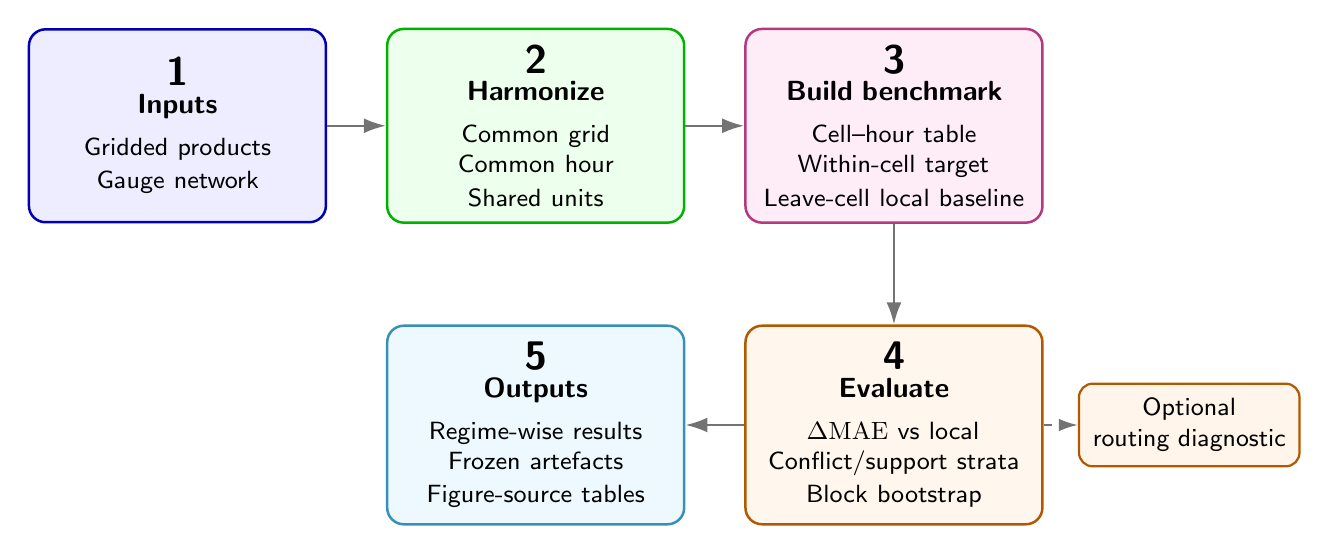
\begin{tikzpicture}[
font=\sffamily,
stage/.style={draw=#1!70!black, fill=#1!7, rounded corners=6pt, line width=0.9pt, text width=3.35cm, minimum width=3.75cm, minimum height=2.45cm, align=center, inner sep=6pt},
arrow/.style={-{Latex[length=2.8mm,width=1.9mm]}, line width=0.9pt, draw=black!55},
branch/.style={-{Latex[length=2.4mm,width=1.6mm]}, line width=0.75pt, dashed, draw=black!55},
note/.style={draw=orange!70!black, fill=orange!8, rounded corners=5pt, line width=0.8pt, text width=2.45cm, minimum width=2.65cm, minimum height=1.05cm, align=center, inner sep=5pt, font=\small\sffamily}
]
\node[stage=blue] (inputs) at (0,0) {{\Large\bfseries 1}\\[-2pt]{\bfseries Inputs}\\[4pt]\small Gridded products\\Gauge network};
\node[stage=green] (harmonize) at (4.55,0) {{\Large\bfseries 2}\\[-2pt]{\bfseries Harmonize}\\[4pt]\small Common grid\\Common hour\\Shared units};
\node[stage=magenta] (build) at (9.10,0) {{\Large\bfseries 3}\\[-2pt]{\bfseries Build benchmark}\\[4pt]\small Cell--hour table\\Within-cell target\\Leave-cell local baseline};

\node[stage=cyan] (outputs) at (4.55,-3.80) {{\Large\bfseries 5}\\[-2pt]{\bfseries Outputs}\\[4pt]\small Regime-wise results\\Frozen artefacts\\Figure-source tables};
\node[stage=orange] (evaluate) at (9.10,-3.80) {{\Large\bfseries 4}\\[-2pt]{\bfseries Evaluate}\\[4pt]\small $\Delta\mathrm{MAE}$ vs local\\Conflict/support strata\\Block bootstrap};
\node[note] (routing) at (12.85,-3.80) {Optional\\routing diagnostic};

\draw[arrow] (inputs.east) -- (harmonize.west);
\draw[arrow] (harmonize.east) -- (build.west);
\draw[arrow] (build.south) -- (evaluate.north);
\draw[arrow] (evaluate.west) -- (outputs.east);
\draw[branch] (evaluate.east) -- (routing.west);
\end{tikzpicture}%
}
\caption{Reproducible geospatial benchmark workflow. The workflow harmonizes heterogeneous precipitation sources, constructs a common cell--hour benchmark with leakage-controlled local baselines, evaluates gridded-source competitiveness by regime, and exports frozen artefacts for manuscript-level regeneration.}
\label{fig:workflow}
\end{figure}

\begin{algorithm}[H]
\caption{Geospatial co-availability benchmark construction.}
\label{alg:benchmark-construction}
\footnotesize
\textbf{Input:} gridded precipitation products; station archive; station-to-cell mapping; evaluation year \(Y\).\\
\textbf{Output:} canonical benchmark table; leave-cell local baselines; conflict strata; bootstrap summaries; frozen artefacts.
\begin{enumerate}
\setlength{\itemsep}{1pt}
\setlength{\parskip}{0pt}
\item Align all gridded products to the target grid and hourly time axis.
\item Assign station observations to grid cells using the station-to-cell mapping.
\item Construct the within-cell gauge target for each candidate cell--hour.
\item Filter to the common evaluable universe with finite target and gridded estimates.
\item Remove same-cell gauges from the station pool used for local prediction.
\item Compute leave-cell IDW local baselines from the remaining nearby gauges.
\item Compute observable source disagreement from pairwise gridded-product differences.
\item For each gridded source \(p\), compute \(\Delta\mathrm{MAE}_{p}=\mathrm{MAE}(p,y)-\mathrm{MAE}(\mathrm{local},y)\).
\item Resample hourly blocks and recompute \(\Delta\mathrm{MAE}_{p}\) intervals.
\item Export frozen artefacts for manuscript-level regeneration and audit checks.
\end{enumerate}
\end{algorithm}

\subsection{Frozen input assets and harmonization}

Analyses use frozen benchmark assets rather than rerunning upstream gridded-product preprocessing. The central intermediate object is a canonical benchmark table with one row per IMERG cell-hour. Its columns include harmonized IMERG, ERA5, and EURADCLIM precipitation estimates, the within-cell AVAMET target aggregate, target-cell support metadata, leakage-controlled leave-cell local baselines, and pairwise source-disagreement metrics used to derive the conflict index. Downstream artefacts are generated from this table and include manuscript tables, block-bootstrap summaries, source-routing diagnostics, and figure-source files. Formal benchmark definitions, bootstrap settings, and regeneration details are consolidated in the supplement, with frozen inputs summarized in Supplementary Table~\ref{tab:supp-repro}.

\subsection{Cell-hour universe construction}

Let \(c\) denote an IMERG grid cell, \(t\) an hourly timestamp in calendar year \(Y\), \(G_{c,t}\) the set of complete AVAMET gauges assigned to cell \(c\) at hour \(t\), \(y_{c,t}^{\mathrm{median}}\) the within-cell target aggregate, and \(x_{c,t}^{p}\) the harmonized estimate from product \(p\). The primary robust-support common universe is
\[
\mathcal{U}_{Y}^{(2)} =
\left\{(c,t):
\begin{aligned}
&y_{c,t}^{\mathrm{median}}\ \text{finite},\quad
x_{c,t}^{\mathrm{IMERG}}\ \text{finite},\quad
x_{c,t}^{\mathrm{ERA5}}\ \text{finite},\\
&x_{c,t}^{\mathrm{EURADCLIM}}\ \text{finite},\quad |G_{c,t}| \ge 2
\end{aligned}
\right\}.
\]
All main 2023 inferential results use \(\mathcal{U}_{2023}^{(2)}\). Positive-rain cases have \(y_{c,t}^{\mathrm{median}}>0\), while the one-gauge universe \(\mathcal{U}_{Y}^{(1)}\) is retained only as a supplementary sensitivity.

\subsection{Within-cell target definition}

The main target is the within-cell median of complete AVAMET gauges in each IMERG cell-hour. This choice was made to obtain a target that is both robust and auditable within the benchmark. Compared with a single-gauge reference, the median better reflects cell-level rainfall support; compared with the mean, it is less affected by isolated station-level extremes. The within-cell mean is retained only as a supplementary target sensitivity reported in Supplementary Table~\ref{tab:supp-target-sensitivity} and Supplementary Table~\ref{tab:supp-support-degradation}.

\subsection{Leakage-controlled leave-cell local baselines}

Local baselines are leave-cell IDW estimates reconstructed from frozen AVAMET assets after excluding gauges in the target cell \citep{shepard1968idw,kurtzman2009interpolation}. Excluding same-cell gauges is central to the benchmark design because it prevents direct target-cell leakage into the local predictor while retaining a realistic nearby-observation alternative from the same network. IDW was selected because it provides a transparent and computationally simple way to reconstruct nearby rainfall information from an irregular gauge network without introducing an additional fitted modeling layer. We evaluate nearest-8, nearest-64, and nearest-64-within-15-km variants to span compact-neighborhood, broad-neighborhood, and distance-capped local comparators as workflow sensitivity variants. Main inferential contrasts use the fixed 64-neighbor baseline as a pre-specified primary comparator to maintain a single fixed inferential benchmark across analyses, whereas best-local and alternative-baseline comparisons are confined to the supplement. The estimand is source competitiveness against strong leave-cell local information under co-availability.

\subsection{Source-disagreement and support stratification}

The main regime marker is observable disagreement among IMERG, ERA5, and EURADCLIM. For each canonical cell-hour, the conflict index is defined as the mean pairwise absolute product difference,
\[
\begin{aligned}
\kappa_{c,t} = \frac{1}{3}\big(&
\left|x_{c,t}^{\mathrm{IMERG}} - x_{c,t}^{\mathrm{ERA5}}\right|\\
&+ \left|x_{c,t}^{\mathrm{IMERG}} - x_{c,t}^{\mathrm{EURADCLIM}}\right|\\
&+ \left|x_{c,t}^{\mathrm{ERA5}} - x_{c,t}^{\mathrm{EURADCLIM}}\right|\big).
\end{aligned}
\]
This index is a computational workflow variable: it is stored in the canonical table, used to stratify benchmark results, and reused by the source-routing diagnostic. Low-, mid-, and high-conflict slices were defined using the 75th and 95th percentiles of \(\kappa_{c,t}\) over the evaluated common universe as pre-specified cutoffs to separate a broad low-disagreement majority from a compact disagreement tail while retaining adequate sample size in each slice. Positive-rain intensity slices were defined as pragmatic hourly evaluation bands spanning light, moderate, heavy, and very heavy rainfall. The slices are 0.1--1 mm, 1--5 mm, 5--10 mm, 10--20 mm, and \(>20\) mm. Support-aware summaries use target-cell gauge availability and support-gradient diagnostics reported in Supplementary Fig.~\ref{fig:supp-support-gradient} and Supplementary Table~\ref{tab:supp-support-gradient}.

The same conflict representation is also used as a diagnostic example of how the benchmark can be converted into an auditable source-routing policy and stress-tested under year-to-year composition shift. We evaluate a simple conflict-gated source-selection rule on the 2022 robust-support universe and apply it unchanged to 2023. The rule uses a pre-specified 75th-percentile conflict gate and selects the lowest-MAE source on each side of the gate among IMERG, ERA5, EURADCLIM, and the fixed leave-cell local benchmark; alternative simple gates are reported in Supplementary Table~\ref{tab:supp-routing-baselines}, and rolling one-year-ahead checks in Supplementary Fig.~\ref{fig:supp-conflict-policy-multiyear-mae} and Supplementary Table~\ref{tab:supp-conflict-policy-multiyear}.

\subsection{Block-bootstrap uncertainty estimation}

The primary metric is MAE, summarized in the main text as gridded-minus-local \deltamae{} against the fixed 64-neighbor benchmark. Uncertainty is estimated with hour-block bootstrap over yearly timestamps \citep{kunsch1989bootstrap}; day-block sensitivities are reported in Supplementary Table~\ref{tab:supp-block-bootstrap}. Main results target cell-hour comparisons under co-availability and ask how gridded products fare when strong local evidence is already available.

\subsection{Reproducibility package and artefact structure}

Manuscript regeneration uses frozen assets summarized in Supplementary Table~\ref{tab:supp-repro}; rebuilding AVAMET-derived assets from raw holdings requires the underlying AVAMET files. The reproducibility package is intended to regenerate manuscript-level tables, figures, and benchmark summaries from frozen inputs, with public scripts, configuration files, result tables, bootstrap summaries, figure-source tables, and the canonical cell--hour table separated from restricted upstream station holdings. Table~\ref{tab:computational-artefacts} summarizes the artefacts exposed by the workflow and their availability.

\begin{table}[t]
\centering
\begin{threeparttable}
\caption{Computational artefacts and availability for manuscript regeneration.}
\label{tab:computational-artefacts}
\footnotesize
\begin{tabularx}{\textwidth}{>{\raggedright\arraybackslash}p{4.0cm} >{\raggedright\arraybackslash}p{4.1cm} >{\raggedright\arraybackslash}X}
\toprule
Artefact & Availability & Role in regeneration \\
\midrule
Canonical cell--hour table & Public derived/frozen asset & Aligned benchmark universe for main analyses \\
Frozen result tables & Public derived/frozen assets & Manuscript tables \\
Bootstrap summaries & Public derived/frozen assets & Uncertainty intervals \\
Figure-source tables & Public derived/frozen assets & Figure regeneration \\
Scripts and configuration files & Public & Reruns from frozen inputs \\
AVAMET raw holdings & Restricted & Upstream reconstruction of station-derived layers \\
Derived benchmark assets & Available on request / subject to source-data conditions & Leave-cell local baselines and AVAMET-derived benchmark layers \\
\bottomrule
\end{tabularx}
\end{threeparttable}
\end{table}

\subsection{Computational design choices and non-routine elements}

Several design decisions in the workflow depart from conventional validation practice and are worth making explicit for reproducibility and transfer.

\textbf{Canonical cell--hour table.} All analyses operate on a single denormalized table with one row per evaluable IMERG cell-hour. This object stores harmonized gridded estimates, the within-cell gauge target, leave-cell local baselines, support metadata, and the pairwise conflict index as co-located columns. Keeping these as co-located columns rather than computing them on demand at analysis time makes every filtering and stratification decision traceable to a single versioned input.

\textbf{Leakage-controlled leave-cell comparator.} Same-cell gauges are removed from the station pool before local IDW prediction. This exclusion is non-trivial: including same-cell gauges in the local predictor would make the comparator a near-interpolant of the target and systematically understate local error. The leave-cell constraint ensures that the local baseline represents information a practitioner could realistically use without prior knowledge of the target cell's own gauge readings.

\textbf{Conflict and support metadata as first-class variables.} The conflict index $\kappa_{c,t}$ and target-cell support count $|G_{c,t}|$ are computed once and stored as columns in the canonical table. Downstream analyses stratify on these stored values rather than recomputing them, which prevents inconsistencies between filtering rules and reported strata definitions.

\textbf{Hour-block bootstrap regeneration.} Uncertainty intervals are computed by resampling over hourly timestamps with a fixed random seed. Seeded bootstrap summaries are exported as frozen artefacts alongside the canonical table, so uncertainty intervals in the manuscript can be regenerated exactly from public inputs without rerunning the full evaluation pipeline.

\textbf{Figure-source artefacts.} Every manuscript figure is generated from a dedicated frozen CSV table in the public repository. This separation between computation and visualization means figure appearance can be audited or adjusted without rerunning upstream analyses, and each visual claim is directly traceable to a named, versioned data file.

\textbf{Conflict-gated routing as an auditable policy object.} The source-routing diagnostic is expressed as a threshold rule applied to stored conflict values rather than as a learned model. Using a pre-specified rule defined on one year and applied unchanged to a second year makes the routing logic fully inspectable and its sensitivity to annual composition shift directly testable.

\section{Results}

The results are organized around five framework diagnostics: how aggregate rankings change under rain-active conditioning, how observable conflict separates screening from cross-checking regimes, how the low-conflict advantage depends on dry-hour composition, how local support changes benchmark difficulty, and how conflict-gated routing behaves under annual composition shift.

\subsection{Global and regime-specific rankings}

The aggregate comparison provided the first diagnostic: a global ranking summarized performance but did not explain where each source was useful. In the all-hours slice, gridded-minus-local \deltamae{} ranged from about +0.02 to +0.06 across products, with bootstrap 95\% intervals excluding zero throughout (Table~\ref{tab:main-inferential}; Figure~\ref{fig:global-positive}). These contrasts are modest in absolute units but non-trivial relative to the local benchmark's own global MAE of about 0.04 mm. When the same comparison was restricted to positive-rain hours, \deltamae{} increased to roughly +0.52 to +0.92 across products, showing that the global result blends weak-signal and rain-active regimes. The gridded-source ranking also changed across regimes: EURADCLIM performed best in the overall slice, IMERG in low and mid conflict, and ERA5 in the conflict tail. Across positive-rain intensity slices the best-performing gridded source also changed (Supplementary Table~\ref{tab:supp-best-eo}; Supplementary Fig.~\ref{fig:supp-best-eo}). Relative-scale, best-local, and alternative-comparator checks reported in Supplementary Table~\ref{tab:supp-relative-scale}, Supplementary Table~\ref{tab:supp-best-eo}, and Supplementary Table~\ref{tab:supp-benchmark-sensitivity} point in the same direction, indicating that the framework-level contrast is not driven by the inferential comparator alone.

\begin{table}[t]
\centering
\begin{threeparttable}
\caption{Main all-hours and positive-rain contrasts against the fixed 64-neighbor leave-cell local benchmark in the two-or-more-gauge subset.}
\label{tab:main-inferential}
\scriptsize
\setlength{\tabcolsep}{4pt}
\begin{tabular}{lcccc}
\toprule
Gridded product & Global \deltamae{} & 95\% CI & Positive-rain \deltamae{} & 95\% CI \\
\midrule
ERA5 & +0.0234 & [+0.0199, +0.0271] & +0.5203 & [+0.4528, +0.5885] \\
EURADCLIM & +0.0206 & [+0.0169, +0.0247] & +0.6895 & [+0.5919, +0.8091] \\
IMERG & +0.0554 & [+0.0493, +0.0618] & +0.9204 & [+0.8221, +1.0187] \\
\bottomrule
\end{tabular}
\end{threeparttable}
\end{table}

\begin{figure}[t]
\centering
\trimtitlegraphic{0.92\textwidth}{figure_1_global_positive_rain_v2.pdf}
\caption{Global and positive-rain MAE contrasts of the three gridded products against the fixed leave-cell local benchmark. Points show \deltamae{} \(=\) gridded product \(-\) local benchmark for IMERG, ERA5, and EURADCLIM in the two-or-more-gauge subset. The all-hours slice gives a compact aggregate ranking, whereas the positive-rain slice reveals a much larger rain-active contrast. Error bars indicate hour-block bootstrap 95\% intervals over 2023 timestamps.}
\label{fig:global-positive}
\end{figure}

\subsection{Conflict separates screening and cross-checking regimes}

Observable inter-product disagreement provided the second diagnostic by separating weak-signal screening conditions from more demanding cross-checking conditions. In the low-conflict slice, all three gridded products showed small negative \deltamae{} values of about -0.009 against the fixed leave-cell local benchmark. In mid conflict the sign reversed for all three products, and in high conflict \deltamae{} rose to about +0.49 for ERA5 and EURADCLIM and above +1.2 for IMERG (Table~\ref{tab:conflict-inferential}; Figure~\ref{fig:conflict}). Computationally, this pattern identifies a broad low-disagreement regime in which broad-coverage fields can support first-pass screening, and higher-disagreement regimes in which local-reference cross-checking becomes more important. Because conflict is constructed from the same products being compared, this stratification is descriptive and diagnostic rather than exogenous.

\begin{table}[t]
\centering
\begin{threeparttable}
\caption{Conflict-conditioned contrasts relative to the fixed 64-neighbor leave-cell local benchmark in the two-or-more-gauge subset.}
\label{tab:conflict-inferential}
\footnotesize
\begin{tabular}{lcc}
\toprule
Gridded product & \deltamae{} & 95\% CI \\
\midrule
\multicolumn{3}{l}{\textbf{Low conflict}} \\
IMERG & -0.0089 & [-0.0105, -0.0075] \\
ERA5 & -0.0088 & [-0.0103, -0.0073] \\
EURADCLIM & -0.0088 & [-0.0103, -0.0073] \\
\addlinespace[3pt]
\multicolumn{3}{l}{\textbf{Mid conflict}} \\
IMERG & +0.0038 & [+0.0015, +0.0060] \\
EURADCLIM & +0.0112 & [+0.0088, +0.0135] \\
ERA5 & +0.0276 & [+0.0252, +0.0300] \\
\addlinespace[3pt]
\multicolumn{3}{l}{\textbf{High conflict}} \\
ERA5 & +0.4916 & [+0.4395, +0.5463] \\
EURADCLIM & +0.5018 & [+0.4403, +0.5650] \\
IMERG & +1.2353 & [+1.1436, +1.3232] \\
\bottomrule
\end{tabular}
\end{threeparttable}
\end{table}

\begin{figure}[t]
\centering
\trimtitlegraphic{0.92\textwidth}{figure_2_conflict_regimes_v2.pdf}
\caption{Conflict-conditioned MAE contrasts of the three gridded products against the fixed leave-cell local benchmark. Points show \deltamae{} \(=\) gridded product \(-\) local benchmark across the low-conflict, mid-conflict, and high-conflict slices defined from the observable disagreement index. Small negative \deltamae{} values appear only in the low-conflict slice, where the regime is diagnostically relevant mainly as a first-pass screening regime. The sign reverses under mid conflict and turns into large positive contrasts in the conflict tail, identifying regimes where local-reference cross-checking becomes more important. Error bars indicate hour-block bootstrap 95\% intervals over 2023 timestamps.}
\label{fig:conflict}
\end{figure}

\subsection{Dry-hour composition of the low-conflict advantage}

The third diagnostic is compositional. The low-conflict slice was overwhelmingly dry, with wet share below 0.3\% (Supplementary Fig.~\ref{fig:supp-conflict-intensity}), so its small all-hours advantage reflects weak-signal composition rather than rain-active source behavior. Within positive-rain cases, all three gridded products showed positive \deltamae{} in every conflict regime, confirming that the low-conflict gain does not transfer to rain-active estimation. This does not make the regime irrelevant: because low conflict covers the bulk of routine cell-hour volume, adequate broad-coverage behavior in this slice can still help triage attention toward the smaller set of rain-active or disagreement-heavy situations where local-reference evidence matters most. Incremental, positive-rain, and day-block sensitivities reported in Supplementary Fig.~\ref{fig:supp-positive-conflict}, Supplementary Fig.~\ref{fig:supp-conflict-incremental}, and Supplementary Table~\ref{tab:supp-block-bootstrap} preserved the same interpretation.

\subsection{Local support hardens the benchmark}

The fourth diagnostic concerns local support. Table~\ref{tab:support-stress} reports $\Delta$MAE across three gauge-support tiers constructed from the existing support-score stratification as a proxy for effective gauge density. All-hours $\Delta$MAE shows no consistent trend across tiers, consistent with dry-hour composition dominating the aggregate. Rain-active $\Delta$MAE, however, increases strictly with support level for all three gridded products: ERA5 rises from $+0.39$ to $+0.52$ to $+0.61$~mm, EURADCLIM from $+0.36$ to $+0.69$ to $+0.85$~mm, and IMERG from $+0.73$ to $+0.92$ to $+1.04$~mm as the density tier goes from low to medium to high. Denser local support therefore hardens the benchmark rather than narrowing the gridded-vs-local gap, converting the conditional nature of the benchmark from a limitation into a quantifiable property: the denser the co-available gauge network, the more demanding the local baseline becomes. Supplementary analyses are reported in Supplementary Table~\ref{tab:supp-support-degradation}, Supplementary Fig.~\ref{fig:supp-support-gradient}, and Supplementary Table~\ref{tab:supp-support-gradient}.

\begin{table}[t]
\centering
\begin{threeparttable}
\caption{Gauge-support stress test: gridded-minus-local $\Delta$MAE across three support tiers. Rain-active $\Delta$MAE increases monotonically with gauge support for all three gridded products, confirming that a denser local network hardens the benchmark rather than narrowing the gap.}
\label{tab:support-stress}
\footnotesize
\setlength{\tabcolsep}{4pt}
\begin{tabular}{lrrcccc}
\toprule
Support tier & $n_\text{all}$ & $n_\text{rain}$ & \multicolumn{2}{c}{Best gridded (all hours)} & \multicolumn{2}{c}{Best gridded (rain-active)} \\
\cmidrule(lr){4-5}\cmidrule(lr){6-7}
& & & Product & $\Delta$MAE & Product & $\Delta$MAE \\
\midrule
\textbf{Low} (${\geq}1$ gauge, score ${\leq}0.34$) & 545,448 & 11,858 & EURADCLIM & $+0.016$ & EURADCLIM & $+0.359$ \\
\textbf{Medium} (${\geq}2$ gauges, all scores) & 882,999 & 20,652 & EURADCLIM & $+0.021$ & ERA5 & $+0.520$ \\
\textbf{High} (${\geq}2$ gauges, score ${>}0.67$) & 561,301 & 11,197 & EURADCLIM & $+0.020$ & ERA5 & $+0.607$ \\
\bottomrule
\end{tabular}
\begin{tablenotes}
\footnotesize
\item $\Delta$MAE = gridded $-$ leave-cell local (fixed 64-neighbour IDW), mm. Low tier uses the broad ${\geq}1$ gauge universe with single-station-like support score (${\leq}0.34$); Medium tier is the main robust-support universe (${\geq}2$ gauges, all scores); High tier restricts further to three-plus-like support scores ($> 0.67$). All-hours $\Delta$MAE shows no consistent trend across tiers, consistent with dry-hour composition dominating the aggregate; rain-active $\Delta$MAE is strictly increasing for all three gridded products.
\end{tablenotes}
\end{threeparttable}
\end{table}

\subsection{Source-routing diagnostic under composition shift}

The fifth diagnostic uses conflict-gated routing to test whether regime information can be converted into an auditable policy object. A policy trained in 2022 selected IMERG below the training-year 75th-percentile conflict threshold and the fixed leave-cell local benchmark otherwise. Applied unchanged to 2023, it used the local branch on 17.5\% of robust-support cell-hours and reduced overall MAE to 0.0328, lower than the fixed leave-cell local benchmark (0.0400) and the best fixed gridded source, EURADCLIM (0.0606). This all-hours gain did not carry over cleanly to positive-rain cases, where MAE did not improve relative to always-local source selection. The 2022$\rightarrow$2023 transfer also exposed annual composition sensitivity: under the same protocol, wet share fell from 5.7\% in 2022 to 2.3\% in 2023 (Supplementary Table~\ref{tab:supp-year-sensitivity}), so the held-out year was materially drier. The routing result therefore validates the diagnostic use of the framework while showing why policy performance must be stress-tested under year-to-year composition shift. Supplementary alert and block-sensitivity checks are reported in Supplementary Table~\ref{tab:supp-conflict-policy-alerts} and Supplementary Table~\ref{tab:supp-conflict-policy-csi-block}; spatial, alternative-routing, and rolling one-year-ahead checks are reported in Supplementary Fig.~\ref{fig:supp-conflict-policy-spatial}, Supplementary Table~\ref{tab:supp-routing-baselines}, and Supplementary Table~\ref{tab:supp-conflict-policy-multiyear}.

\subsection{Ablation: what each workflow design decision contributes}

Table~\ref{tab:ablation} traces how the apparent product ranking and the resulting operational conclusion change as each design element is added to the simplest possible benchmark. Version~A computes raw gridded MAE against the gauge target across all hours with no local comparator. This produces a single global ranking in which EURADCLIM appears best (MAE\,=\,0.061~mm). Versions B and C show that the ranking is not stable: adding a positive-rain filter reveals that ERA5 outperforms EURADCLIM in rain-active hours (MAE\,=\,1.55 vs.\ 1.72~mm), and adding conflict stratification introduces a further regime dependency in which the apparent winner changes between conflict bins. Together, Versions A--C demonstrate that a global ranking conflates multiple regimes and that the choice of conditioning already changes the stated conclusion.

Version~D is the design-critical transition. Introducing a leakage-controlled leave-cell local comparator and expressing performance as $\Delta$MAE~=~gridded~$-$~local reverses the framing: all three gridded products are worse than the dense-gauge local baseline in both all-hours ($\Delta > 0$, smallest gap EURADCLIM at $+0.019$~mm) and rain-active conditions ($\Delta \gg 0$, ERA5 closest at $+0.47$~mm), even using the broad ${\geq}1$ gauge universe. The question shifts from which product is best to when the local reference dominates and when a gridded layer adds value in its place. Version~E shows that tightening the support filter to $|G_{c,t}| \geq 2$ gauges reduces the evaluable universe by 38\% (from 1.4M to 883k cell-hours) and widens both gaps ($\Delta_\text{all} = +0.021$, $\Delta_\text{rain} = +0.52$~mm), consistent with the finding that a more robust local target is harder to match. Finally, Version~F shows that conflict-gated routing---the full workflow---exploits the low-conflict screening regime to reduce all-hours MAE by 18\% relative to always-local (0.033 vs.\ 0.040~mm) while correctly identifying that the rain-active regime still favours the local branch.

The table makes the workflow argument concrete: removing any single design decision produces a materially different apparent winner or operational conclusion. The ranking instability across Versions A--C is not a sign of model failure; it is the intended diagnostic signal that a global average conceals.

\begin{table}[t]
\centering
\begin{threeparttable}
\caption{Ablation study: effect of each workflow design decision on product rankings. Each version adds one element to the previous design. Best-ranked product (all-hours and rain-active) and the resulting operational conclusion are shown for each design.}
\label{tab:ablation}
\footnotesize
\setlength{\tabcolsep}{4pt}
\begin{tabular}{clp{3.1cm}cp{2.8cm}cp{4.4cm}}
\toprule
Ver. & Design element added & Best (all hours) & Metric & Best (rain-active) & Metric & Operational conclusion \\
\midrule
\textbf{A} & Raw MAE vs.\ target, all hours, no local comparator & EURADCLIM & $0.061$ & ERA5 & $1.55$ & Single-number ranking; EURADCLIM preferred globally \\
\addlinespace[2pt]
\textbf{B} & $+$ positive-rain conditioning & EURADCLIM & $0.061$ & ERA5 & $1.55$ & Ranking shifts in rain-active hours (ERA5 $\neq$ EURADCLIM) \\
\addlinespace[2pt]
\textbf{C} & $+$ conflict stratification (no local) & IMERG / IMERG / ERA5\textsuperscript{\dag} & varies & Regime-dependent & varies & No stable winner; apparent best changes with conflict regime \\
\addlinespace[2pt]
\textbf{D} & $+$ leave-cell local comparator ($\Delta$MAE), support ${\geq}1$ & All worse; EURADCLIM closest & $\Delta=+0.019$ & All worse; ERA5 closest & $\Delta=+0.47$ & All gridded products inferior to local; question shifts from ranking to when local evidence dominates \\
\addlinespace[2pt]
\textbf{E} & $+$ support ${\geq}2$ gauge filter & EURADCLIM (lowest $\Delta$) & $\Delta=+0.021$ & ERA5 (lowest $\Delta$) & $\Delta=+0.52$ & Support filter reduces universe (1.4M$\to$883k cell-hours) and widens gridded-minus-local gap; direction preserved \\
\addlinespace[2pt]
\textbf{F} & $+$ conflict-gated routing (full workflow) & Hybrid routing & $0.0328$ & Local-always & $1.026$ & Routing reduces all-hours MAE by 18\% vs.\ always-local; positive-rain still needs local branch \\
\addlinespace[2pt]
\bottomrule
\end{tabular}
\begin{tablenotes}
\footnotesize
\item[\dag] Low/mid/high conflict bins respectively (IMERG best in low and mid; ERA5 best in high conflict).
\item Versions A--C use raw MAE vs.\ the gauge target. Versions D--F use $\Delta$MAE = gridded $-$ local (leave-cell IDW). Version~D uses the broad ${\geq}1$ gauge universe ($n=1{,}428{,}447$; 32{,}510 positive-rain); Version~E--F use the robust ${\geq}2$ gauge universe ($|\mathcal{U}_{2023}^{(2)}|=882{,}999$; 20{,}652 positive-rain). MAE in mm.
\end{tablenotes}
\end{threeparttable}
\end{table}

\section{Discussion}

\subsection{What the benchmark reveals in the eastern Spain case study}

The ablation in Table~\ref{tab:ablation} organizes the case-study findings as a sequence of design decisions rather than as a list of product properties. Its central message is that no single design decision is cosmetic: removing any one of them changes the apparent winner or the operational conclusion. The key transition is Version~C~$\to$~D: products that appear adequate in a global or conflict-conditioned raw-MAE comparison all become inferior to the leave-cell local baseline once that baseline is introduced. This is not a failure of the gridded products; it is a consequence of what the benchmark is actually measuring once co-availability is taken seriously.

The conflict and support structure identified in Results is best read as a diagnostic about when the local branch is worth activating, not as a fixed product catalogue. Low-conflict hours cover the bulk of the evaluable universe and their modest all-hours gridded advantage is largely a dry-hour composition effect, as the ablation's Version B shows (rain-active ERA5 overtakes EURADCLIM immediately upon conditioning). The conflict-gated routing experiment in Version~F quantifies the operational implication: exploiting the low-conflict screening regime reduces all-hours MAE by 18\% relative to always-local, while preserving the local branch for rain-active conditions where gridded products consistently underperform. This reading is consistent with broader literature on context dependence and regime sensitivity in gridded precipitation evaluation \citep{kidd2011status,maggioni2018review,derin2016complexterrain,yu2020highdensity,tessema2020representativeness,tian2018gaugedensity,tozer2012proxy,porcu2014uncertainties,peino2024westernmed,gomiscebolla2023spain}.

\subsection{What the workflow contributes as a computational geoscience protocol}

The transferable object is the benchmark protocol: the data model, filtering rules, leakage-controlled comparator construction, disagreement stratification, and reproducibility package. This emphasis aligns with reproducible geoscience and workflow-oriented scientific computing, where reusable data products, transparent processing steps, and executable regeneration paths are part of the scientific contribution \citep{pebesma2012rgeoscience,gil2016geosciencepaper,wilson2017goodenough,nuest2021practical}. The protocol converts heterogeneous satellite, radar-derived, reanalysis, and station sources into a common hourly cell--hour evaluation table; defines an explicit within-cell gauge target; removes same-cell gauges from local predictors; compares gridded sources against fixed leave-cell baselines; stratifies results by rain activity, support, and observable source disagreement; and exports frozen artefacts for manuscript-level regeneration.

This separation between case-study findings and methodological contribution is important. The case-study ranking is local, but the computational design is portable to domains where multiple gridded products are co-available, local observations can support a defensible leave-cell comparator, and users need to distinguish broad-coverage screening from rain-active local-reference branching. In that sense, the study contributes an auditable geospatial benchmarking workflow rather than a product catalogue. It brings remote sensing and reanalysis products, dense field measurements, local interpolation, conflict diagnostics, bootstrap uncertainty, and reproducibility assets into a common evaluative framework \citep{pohl1998datafusion,refsgaard2007uncertainty,bennett2013performance,kirschbaum2017applications,portier2023gpmapplications}. This framing also matters because auditable dense-gauge geospatial benchmarks remain relatively uncommon at larger spatial scales \citep{kidd2017gauges}.

A specific concern with the conflict index is that, being derived from the same products being evaluated, it may function as a proxy for precipitation magnitude rather than as an independent disagreement signal. The evidence here is against this being trivially true. First, the monotonic relationship between conflict stratum and gridded-minus-local $\Delta$MAE --- small negative in low conflict, near-zero in mid, strongly positive in the tail --- holds within rain-active hours as well, where precipitation magnitude is by definition non-zero. Second, the conflict-threshold sweep shows a well-defined optimum at the 80--85th percentile (all-hours MAE 0.0321--0.0323~mm) that degrades on both sides, rather than improving monotonically with a higher threshold as a pure magnitude proxy would predict. Third, the positive-rain $\Delta$MAE increases monotonically with the conflict threshold (from 1.032 at the 50th percentile to 1.187 at the 95th), confirming that the local branch remains better for rain-active cases regardless of the threshold chosen. These patterns support treating the conflict index as a triage diagnostic: an observable marker that stratifies when gridded information is more or less trustworthy relative to local evidence, without requiring it to be an exogenous uncertainty measure.

\subsection{Scope conditions and limitations}

Several limitations bound the interpretation of the case-study findings. First, the analysis is conducted in a single eastern Spain testbed with distinctive coastal and terrain gradients, so the reported effect sizes should not be treated as directly transferable to other hydroclimatic settings. Second, the local comparator is intentionally strong and depends on access to a dense AVAMET network; the benchmark is therefore most informative in domains where a similarly defensible leave-cell local alternative can be constructed. Third, the conflict index is derived from the same gridded products being evaluated and should be interpreted only as an observed stratification marker, not as an exogenous uncertainty measure or a causal explanation of error.

Further limitations concern policy transfer and reproducibility scope. The diagnostic 2022$\rightarrow$2023 source-routing transfer is not composition-matched across years. Under the same protocol, wet share declines from 5.7\% in 2022 to 2.3\% in 2023 (Supplementary Table~\ref{tab:supp-year-sensitivity}), meaning that the held-out year is materially drier. This shift may mechanically improve all-hours MAE and therefore overstate the apparent out-of-sample benefit of a policy that exploits low-conflict screening conditions; the fact that positive-rain MAE does not improve relative to always-local mitigates but does not remove that concern. Manuscript regeneration is supported by public frozen assets, but full end-to-end reconstruction of the AVAMET-derived benchmark layers depends on source holdings that are not publicly available. Finally, the local benchmark family is intentionally simple and reproducible; we do not claim that IDW is the strongest possible local predictor, only that it provides a transparent and computationally interpretable comparator for the benchmarking question posed here.

Taken together, these scope conditions define where the protocol is most informative: dense-support co-availability settings in which target definition, comparator strength, support heterogeneity, and observable source disagreement can be made explicit in the evaluation itself.

\section{Conclusions}

In this eastern Spain testbed, the workflow showed that a single global ranking hides important regime structure. EURADCLIM performed best among gridded products overall, IMERG performed best in low and mid conflict, and ERA5 performed best in the conflict tail, while positive-rain conditioning exposed much larger contrasts than the all-hours aggregate.

The transferable object is the benchmark protocol: the data model, filtering rules, leakage-controlled comparator construction, disagreement stratification, and reproducibility package. This protocol makes conditional competitiveness auditable under co-availability and heterogeneous local support.

For workflows resembling the present setting, gridded products can provide first-pass screening across many quiet low-conflict cell-hours and trigger faster, more selective local-evidence branching once rainfall becomes active or source disagreement increases. The conflict-gated routing experiment illustrates that diagnostic value, while showing that annual composition shift must be part of any policy stress test.

\section*{CRediT authorship contribution statement}

Marc Semper, Manuel Curado, Jose F. Vicent, and Marco Podda: Conceptualization, Methodology, Software, Formal analysis, Validation, Visualization, Writing -- original draft, Writing -- review \& editing. All authors contributed equally to this work.

\section*{Declaration of competing interest}

The authors declare that they have no known competing financial interests or personal relationships that could have appeared to influence the work reported in this paper.

\section*{Funding}

This research did not receive any specific grant from funding agencies in the public, commercial, or not-for-profit sectors.

\section*{Data availability}

The gridded precipitation products analysed in this study are available from the public sources cited in the manuscript. The public GitHub repository contains the versioned analysis scripts, configuration files, canonical cell--hour table, manuscript-level frozen result tables, bootstrap summaries, and figure-source tables used directly in this article. These materials support manuscript-level regeneration from frozen inputs rather than end-to-end reconstruction from raw holdings. The upstream AVAMET source holdings required to reconstruct the AVAMET-derived benchmark assets from scratch are not publicly available. Rebuilding the leave-cell benchmark layer therefore requires access to the AVAMET source holdings. Derived benchmark assets are available from the corresponding author upon reasonable request and subject to any applicable source data-sharing conditions. Supplementary Table~\ref{tab:supp-repro} summarizes the frozen inputs used for manuscript regeneration. The code and configuration files are available at \url{https://github.com/MarcSemperLloret/Conditional-competitiveness-and-conflict-gated-source-selection-of-gridded-precipitation}.

\section*{Declaration of Generative AI and AI-assisted technologies in the manuscript preparation process}

During the preparation of this work, the authors used OpenAI tools to support outlining, phrasing, and language editing of draft text. After using these tools, the authors reviewed and edited the content as needed and take full responsibility for the content of the publication.


\bibliographystyle{elsarticle-num}
\bibliography{references}

\def\includedsupplement{1}
\input{supplement.tex}

\end{document}
